\chapter{Cronograma e custos do projeto}
Um bom planejamento é essencial para o sucesso de um projeto, ainda mais quando trata-se de um trabalho em equipe. Com isso em mente, foi feito um cronograma detalhado já na proposta do GoBike, que pôde ser seguido sem grandes empecilhos, fator este que foi essencial para o sucesso do desenvolvimento. 

\section{Cronograma}

\begin{figure}[!h]
\centering
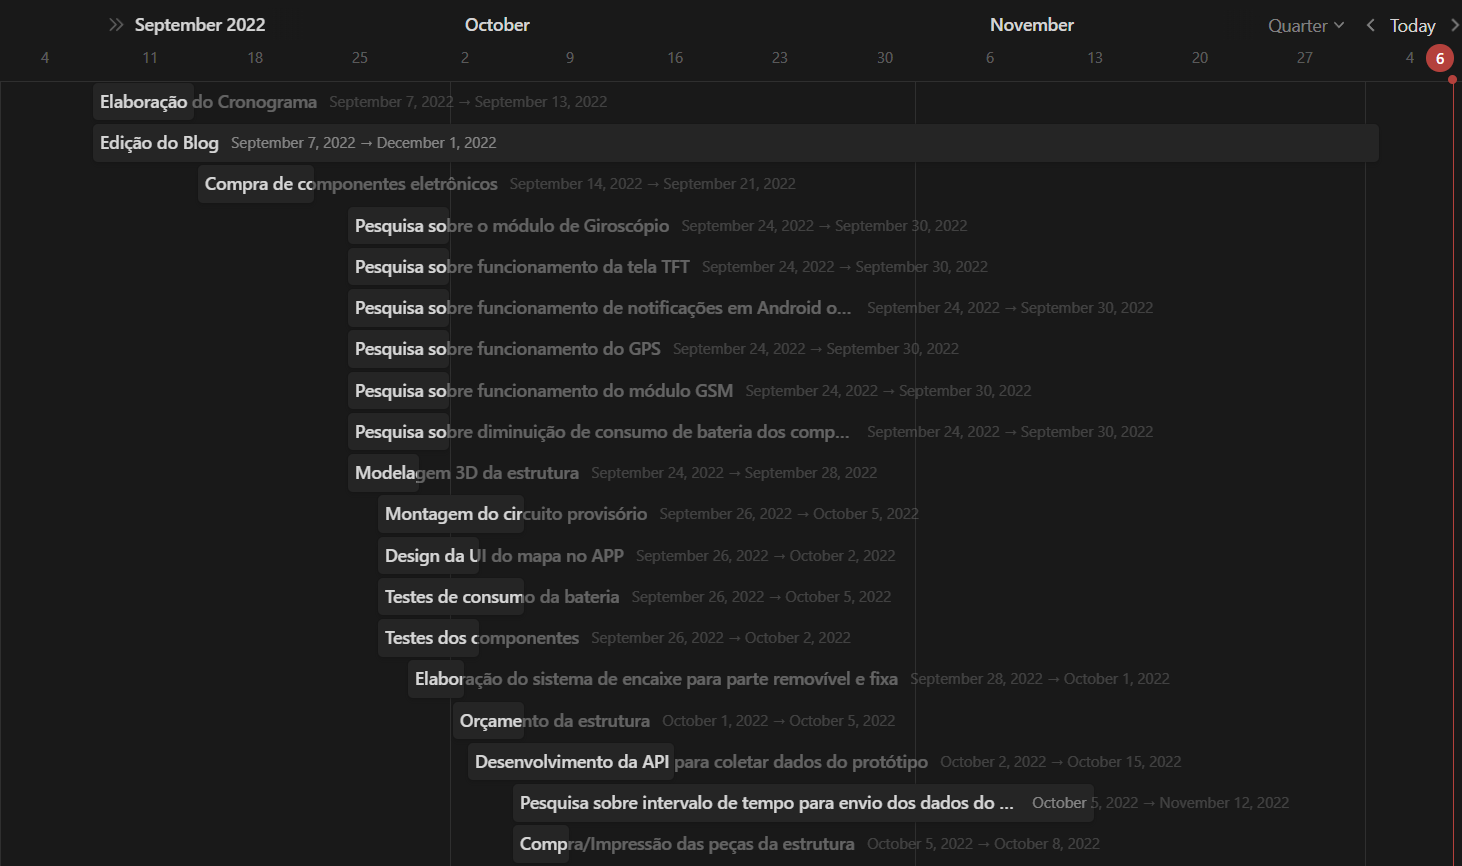
\includegraphics[width=15cm]{capitulos/Figuras/Cronograma1.png}
\caption{Cronograma do projeto (parte 1).}
\label{fig:cronograma_1}
\end{figure}

\newpage

\begin{figure}[!h]
\centering
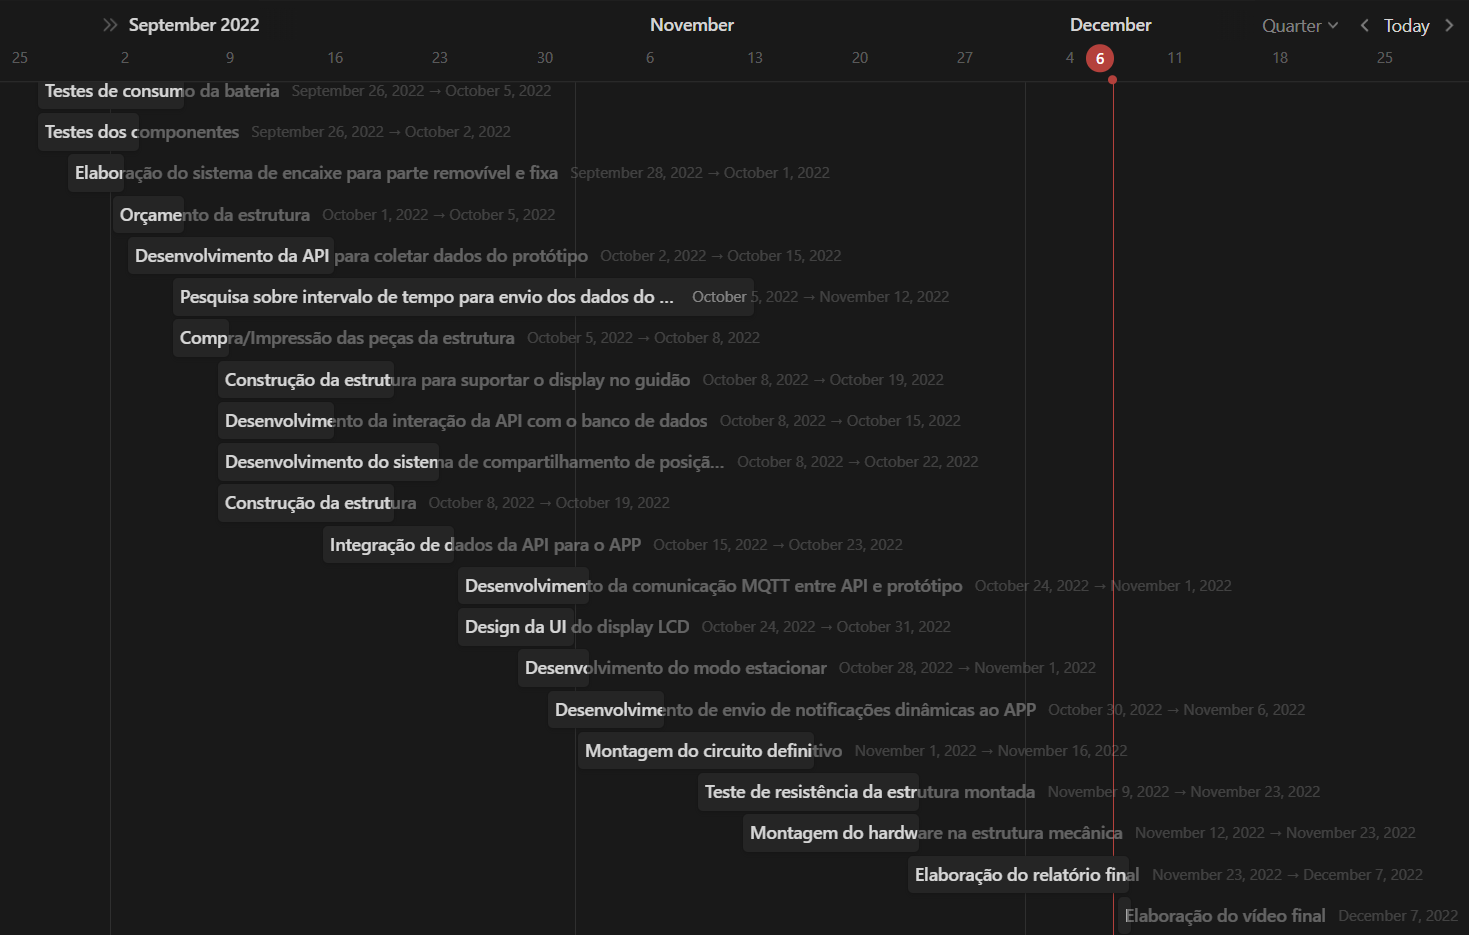
\includegraphics[width=15cm]{capitulos/Figuras/Cronograma2.png}
\caption{Cronograma do projeto (parte 2).}
\label{fig:cronograma_2}
\end{figure}

\section{Custos}

Foram desconsiderados do custo total alguns insumos básicos, como jumpers e estanho. Além disso, componentes que queimaram ou vieram com defeito também não entraram no cálculo, visto que foram imprevistos e, em condições ideais, não aconteceriam. Visto isso, o custo total estimado do projeto seria de aproximadamente R\$436,16, conforme Tabela 1 a seguir. Porém na Tabela 2 temos a lista de componentes completa, incluindo hardwares que foram comprados pra substituir os que queimaram e os que foram usados para teste e acabaram não sendo incorporados no projeto final.

\newpage

\begin{table}[]
\centering
\label{tab:componentes} 
\begin{tabular}{|l|l|l|}
\hline
Qtd. & Nome                               & Preço     \\ \hline
1    & ESP32                              & R\$72,90  \\ \hline
1    & Display OLED 0.96”                 & R\$38,61  \\ \hline
1    & Powerbank 5V 2.1A 10000 mAh        & R\$72,00  \\ \hline
1    & Módulo GSM GPRS SIM800L            & R\$ 56,90 \\ \hline
1    & Acelerômetro e Giroscópio MPU-6050 & R\$ 20,75 \\ \hline
1    & Placa Perfurada 15cmx10cm          & R\$ 10,00 \\ \hline
1    & GPS GY-NEO6MV2                         & R\$ 65,00 \\ \hline
1    & Impressão 3D                       & R\$ 100,00 \\ \hline
     & Valor Total                        & R\$ 436.16 \\ \hline
\end{tabular}
\caption{Lista de componentes}
\end{table}


\begin{table}[]
\centering
\label{tab:componentes2} 
\begin{tabular}{|l|l|l|}
\hline
Qtd. & Nome                               & Preço     \\ \hline
1    & ESP32                              & R\$72,90  \\ \hline
2    & Display OLED 0.96”                 & R\$77,22  \\ \hline
1    & Powerbank 5V 2.1A 10000 mAh        & R\$72,00  \\ \hline
1    & Módulo GSM GPRS SIM800L            & R\$ 56,90 \\ \hline
1    & Acelerômetro e Giroscópio MPU-6050 & R\$ 20,75 \\ \hline
1    & Placa Perfurada 15cmx10cm          & R\$ 10,00 \\ \hline
1    & GPS GY-NEO6MV2                        & R\$ 65,00 \\ \hline
1    & Impressão 3D                       & R\$ 100,00 \\ \hline
2    & LM2596                             & R\$ 30,00  \\ \hline
2    & MT3608                             & R\$ 30,00 \\ \hline
1    & Bateria De LiPo Recarregável 3.7V 1100mAh & R\$ 79,90 \\ \hline
1    & Carregador De Bateria LiPo         & R\$ 49,90 \\ \hline
     & Valor Total                        & R\$ 664,57 \\ \hline
\end{tabular}
\caption{Lista de componentes finais}
\end{table}